\documentclass[aspectratio=169,
hyperref={colorlinks,urlcolor=blue}
]{beamer}


%\usetheme{Pittsburgh}
\usetheme{default}
\usepackage{colortbl}%colored tables
%For using helvetica font:
\usepackage[scaled]{helvet}
\usepackage[T1]{fontenc}
\renewcommand\familydefault{\sfdefault}
\urlstyle{same} %sets the fonts for urls
\usepackage{pdfpages}
\usepackage{siunitx}
\usepackage{caption}
\usepackage{pifont}%for dings
\usepackage{pgfplots}%for 3d plotting
\pgfplotsset{compat = newest}
\usepackage{mathtools}%box in align env \Aboxed
\usepackage[american,smartlabels]{circuitikz}%for drawing circuits
\usepackage{multimedia}
\usepackage{animate}
\usepackage{xcolor}


\usetikzlibrary{arrows}
\usetikzlibrary {3d} 
\usetikzlibrary{decorations.markings, math}
\usetikzlibrary{intersections, pgfplots.fillbetween}
\usetikzlibrary {shapes.geometric} 


%\definecolor{myblue}{RGB}{5, 34, 150}
\definecolor{myblue2}{RGB}{5, 34, 150}
\definecolor{myblue}{RGB}{0,36,82}
\definecolor{myred}{RGB}{207, 2, 13}
\definecolor{mygreen}{RGB}{0, 158, 11}
\definecolor{myyellow}{RGB}{220,220,0}
\definecolor{qblue}{RGB}{0,36,82}
\definecolor{qgold}{RGB}{250,189,15}
\definecolor{qred}{RGB}{185,14,49}
\definecolor{cblue}{rgb}{0.13, 0.67, 0.8}
\definecolor{corange}{rgb}{0.8, 0.34, 0.0}
\definecolor{cpurple}{rgb}{0.54, 0.29, 0.42}

%%%%%%%%%%%% General settings
\setbeamercolor{frametitle}{fg=black}
\setbeamercolor{title}{fg=black}
\setbeamercolor{author}{fg=myblue2}

\beamertemplatenavigationsymbolsempty %no navigation controls at bottom of slides
%\setbeamertemplate{footline}[frame number]
\usefonttheme{professionalfonts} 
\setbeamerfont{title}{series=\bfseries,parent=structure}
\setbeamerfont{frametitle}{series=\bfseries,parent=structure}

%%%%%%%%%%%%Lists
\setbeamertemplate{itemize item}[circle] %{\color{myblue}$\circ$}
\setbeamertemplate{itemize subitem}{\color{myblue2}$\circ$}
\setbeamertemplate{itemize subsubitem}{\color{myblue2}$\cdot$}
\setbeamercolor{itemize item}{bg=myblue2,fg=myblue2}
\setbeamercolor{enumerate item}{bg=myblue2,fg=myblue2}
%%%%%%%%%%%%%%%%%%%%%%%%%%%%

%%%%%%%%%%%%Blocks
\setbeamertemplate{blocks}[rounded]
%Default block
\setbeamercolor{block title}{bg=myblue2, fg=white}
\setbeamercolor{block body}{bg=myblue2!10}
\setbeamerfont{block body}{size=\scriptsize}
\setbeamerfont{block title}{size=\scriptsize}
%Alert block
\setbeamercolor{block title alerted}{bg= myblue2, fg=white}
\setbeamercolor{block body alerted}{bg=myblue2!10}
\setbeamerfont{block body alerted}{size=\scriptsize}
\setbeamerfont{block title alerted}{size=\scriptsize}
%example block
\setbeamercolor{block title example}{bg=mygreen, fg=white}
\setbeamercolor{block body example}{bg=mygreen!10}
\setbeamerfont{block body example}{size=\scriptsize}
\setbeamerfont{block title example}{size=\scriptsize}
%%%%%%%%%%%%%%%%55


%%%%%%%%%%%%Figures and captions
\captionsetup{font=scriptsize,labelfont=scriptsize}
%\setbeamertemplate{caption}{\raggedright\insertcaption\par}
\newenvironment{capfig}[3]{\begin{figure}\includegraphics[width=#1\textwidth]{#2}\caption*{\textit{#3}}\end{figure}}{}

%\makeatother
%\setbeamertemplate{footline}
%{
%  \leavevmode%
%  \hbox{%
%  \begin{beamercolorbox}[wd=.4\paperwidth,ht=2.25ex,dp=1ex,center]{author in head/foot}%
%    \usebeamerfont{author in head/foot}\insertshortauthor
%  \end{beamercolorbox}%
%  \begin{beamercolorbox}[wd=.6\paperwidth,ht=2.25ex,dp=1ex,center]{title in head/foot}%
%    \usebeamerfont{title in head/foot}\insertshorttitle\hspace*{3em}
%    \insertframenumber{} / \inserttotalframenumber\hspace*{1ex}
%  \end{beamercolorbox}
%  }%
%  \vskip0pt%
%}
%\makeatletter

\makeatother
\setbeamertemplate{footline}
{
  \leavevmode%
  \hbox{%
\begin{beamercolorbox}[wd=.27\paperwidth,ht=2.25ex,dp=1ex,center]{author in head/foot}%
    \color{black}{\insertinstitute}
\end{beamercolorbox}
  \begin{beamercolorbox}[wd=.27\paperwidth,ht=2.25ex,dp=1ex,center]{author in head/foot}%
    \color{black}{\inserttitle}
  \end{beamercolorbox}%
  \begin{beamercolorbox}[wd=.27\paperwidth,ht=2.25ex,dp=1ex,center]{title in head/foot}%
    \color{black}{\insertshortauthor}
  \end{beamercolorbox}
  \begin{beamercolorbox}[wd=.27\paperwidth,ht=2.25ex,dp=1ex,center]{title in head/foot}%
    \hspace{.28\paperwidth}\color{black} \insertframenumber{} / \inserttotalframenumber\hspace*{1ex}
  \end{beamercolorbox}
  }%
  \vskip0pt%
}
\makeatletter

\setbeamertemplate{title page}
{
  \begin{tikzpicture}[remember picture,overlay]
    \def\barh{4}%15
  
    \draw[color=myblue2,line width=\barh] ([yshift=-0.5*\barh]current page.north west) -- ([yshift=-0.5*\barh,xshift=-0.67\paperwidth]current page.north east);
    \draw[color=myblue2,line width=\barh] ([yshift=-0.5*\barh,xshift=-0.67\paperwidth]current page.north east) -- ([yshift=-0.5*\barh,xshift=-0.34\paperwidth]current page.north east);
    \draw[color=myblue2,line width=\barh] ([yshift=-0.5*\barh,xshift=-0.34\paperwidth]current page.north east) -- ([yshift=-0.5*\barh]current page.north east); 
  
    \draw[color=myblue2,line width=\barh] ([yshift=0.5*\barh]current page.south west) -- ([yshift=0.5*\barh,xshift=-0.67\paperwidth]current page.south east);
    \draw[color=myblue2,line width=\barh] ([yshift=0.5*\barh,xshift=-0.67\paperwidth]current page.south east) -- ([yshift=0.5*\barh,xshift=-0.34\paperwidth]current page.south east);
    \draw[color=myblue2,line width=\barh] ([yshift=0.5*\barh,xshift=-0.34\paperwidth]current page.south east) -- ([yshift=0.5*\barh]current page.south east);
    %\node[left] at (current page.east) {
    %
\includegraphics[scale=0.1]{figures/coverpage}
    %};
  \end{tikzpicture}
  
  \usebeamerfont{title}\usebeamercolor[fg]{title}\inserttitle\par
  \usebeamerfont{subtitle}\usebeamercolor[fg]{subtitle}\insertsubtitle\par
  \vspace{2cm}
  \usebeamerfont{author}\usebeamercolor[fg]{author}\insertauthor\par
  \usebeamerfont{institute}\usebeamercolor[fg]{author}\insertinstitute\par
  \usebeamercolor[fg]{author}\par
  \usebeamercolor[fg]{titlegraphic}\inserttitlegraphic

} 

\setbeamertemplate{frametitle}{%
    \nointerlineskip%
        \par\hspace*{-\dimexpr0.5\paperwidth-0.5\textwidth}\textcolor{myblue2}{\rule{0.33\paperwidth}{6pt}}\textcolor{myblue2}{\rule{0.33\paperwidth}{6pt}}\textcolor{myblue2}{\rule{0.34\paperwidth}{6pt}} 
    \begin{beamercolorbox}[wd=\paperwidth,ht=0.75cm,dp=0.6ex]{frametitle}
        \hspace*{0.5cm}\strut\usebeamerfont{frametitle}\insertframetitle\strut
        %\hrule
    \end{beamercolorbox}%
    %%Line below:
%\par\hspace*{-\dimexpr0.5\paperwidth-0.5\textwidth}\textcolor{myblue}{\rule{\paperwidth}{0.4pt}}
     % <-- calculation of left margin width + rule
     %\textcolor{red}{\noindent\rule{\paperwidth}{2pt}}
}


%%%%%%%%%%%%Frame templates

%Slide with title
\newenvironment{titleframe}[1]
{\begin{frame}\frametitle{#1}\end{frame}}
{}

%Slide with title and itemize list:
\newenvironment{bulletframe}[1]
{\begin{frame}{#1} \itemize}
{\enditemize \end{frame}}

%Slide with two columns 50/50
\newenvironment{twocolframe}[3]
{\begin{frame}{#1}
 \begin{columns}[T]
 \column{0.5\textwidth}#2
 \column{0.5\textwidth}#3
 \end{columns}\end{frame}}{}

%Slide with two columns 60/40 <<<<<<<<<<<<<<<<<<<<<<  This one!
\newenvironment{twocolframesf}[3]
{\begin{frame}{#1}
 \begin{columns}[T]
 \column{0.6\textwidth}#2
 \column{0.4\textwidth}#3
 \end{columns}\end{frame}}{}
 
%Slide with two columns 70/30
\newenvironment{twocolframest}[3]
{\begin{frame}{#1}
 \begin{columns}[T] 
 \column{0.7\textwidth}#2
 \column{0.3\textwidth}#3
 \end{columns}\end{frame}}{} 
 
%Slide with two columns 40/60
\newenvironment{twocolframefs}[3]
{\begin{frame}{#1}
 \begin{columns}[T] 
 \column{0.4\textwidth}#2
 \column{0.6\textwidth}#3
 \end{columns}\end{frame}}{}
 
%Slide with two columns 70/30
\newenvironment{twocolframets}[3]
{\begin{frame}{#1}
 \begin{columns}[T] 
 \column{0.3\textwidth}#2
 \column{0.7\textwidth}#3
 \end{columns}\end{frame}}{} 

 
%Colloquium speaker (title, abstract, picture file, speaker name)
\newenvironment{colloquium}[5]
{
\begin{frame}{Colloquium: Friday 1:30pm in Stirling A}
\begin{columns}[T] 
 \column{0.8\textwidth}
 \textbf{#1}\\
 #2
 \column{0.2\textwidth}
 \capfig{#3}{#4}{#5}
 \end{columns}
\end{frame}
}
{} 

%%%%%%%%%%%%%Set Hyperref colors


\hypersetup{
  colorlinks=true,
  linkcolor=blue,    
  urlcolor=blue,     
  citecolor=blue      
}
%%%%%%%%%%%%%TOC bolding
\setbeamerfont{section in toc}{series=\bfseries}



%Frames:
% \twocolframesf 60/40 (fs, st, ts) 
% \titleframe
% bulletframe


%%%%%%%%%%%%%%%%%%%%%%%%%
%%%%%% START OF PRESENTATION %%%%%%
%%%%%%%%%%%%%%%%%%%%%%%%%

\title{Simple Harmonic Motion}
\institute{Form, Examples and Modelling}
\author{Building Models to Describe our World}


\begin{document}

%%%%%%%%%%%%%%%%%%%%%%%%%
%%%%%% Title slide %%%%%%
%%%%%%%%%%%%%%%%%%%%%%%%%
\begin{frame}
\titlepage
\thispagestyle{empty}

\begin{textblock*}{5cm}(11cm,4cm)
    
\includegraphics[width=4cm]{../figures/BMDW/logo}
\end{textblock*}

\end{frame}

%%%%%%%%%%%%%TOC

\twocolframe{Outline}
{\tableofcontents[sections=1-2, subsectionstyle=show/show]}
{\tableofcontents[sections=3, subsectionstyle=show/show]}

%%%%%%%%%%%%%%%%%%%%%%%%%











%%%%%%%%%%%%%%%%%%%%%%%%%%%%%%%%
\section{The Structure of SHM}
\label{sec:shhstructure}
\title{The Structure of SHM}
\institute{Simple Harmonic Motion}
\author{\insertsubsection}


%%%%%%%%%%%%%%%%%%%%%%%%%
\begin{frame}
\titlepage
\thispagestyle{empty}
\end{frame}

%%%%%%%%%%%%%%%%%%%%%%%%









%%%%%%%%%%%%%%%%%%%%%%%%%%%
\subsection{The Concept and Formula}
\label{subsec:conceptandformulashm}
\begin{frame}{Simple Harmonic Motion}
\begin{itemize}
\item Anytime that you have this equation of motion:
\begin{align*}
\frac{d^2x}{dt^2}=-\omega^2 x
\end{align*}
\item We call the motion ``Simple Harmonic Motion'' and the solution is:
\begin{align*}
x(t)=A\cos(\omega t +\phi)
\end{align*}
(note that sine also works)
\item Where $A$ and $\phi$ are ``integration constants'' that depend on the specific ``initial conditions''.
\end{itemize}

\end{frame}

%%%%%%%%%%%%%%%%%%%%%%%%%%%%%%%%


%%%%%%%%%%%%%%%%%%%%%%%%%%%%%%%%
\subsection{Application example: spring-mass system}
\label{subsec:springmassexample}
\twocolframesf{Applications of SHM: spring-mass system}
{
\only<1>{
\begin{itemize}
\item The equation of motion for SHM comes up \textit{a lot} in physics.
\item The most obvious case is to describe the position of a mass attached to a spring:
\begin{align*}
ma&=-kx\\
m\frac{d^2x}{dt^2}&=-k x\\
\therefore \frac{d^2x}{dt^2}&=-\frac{k}{m}x=-\omega^2 x\\
\omega&=\sqrt{\frac{k}{m}}
\end{align*}
\end{itemize}
}
\only<2>{
\begin{itemize}
\item The position as a function of time is given by:
\begin{align*}
x(t)=A\cos(\omega t +\phi)
\end{align*}
\item The velocity as a function of time is given by:
\begin{align*}
v(t)=\frac{dx}{dt}=-A\omega\sin(\omega t +\phi)
\end{align*}
\item Need to determine $A$ and $\phi$ from initial conditions:
\begin{itemize}
\item[$\rightarrow$] Specify (say) position and velocity at $t=0$.
\end{itemize}

\end{itemize}

}
}
{

\begin{center}
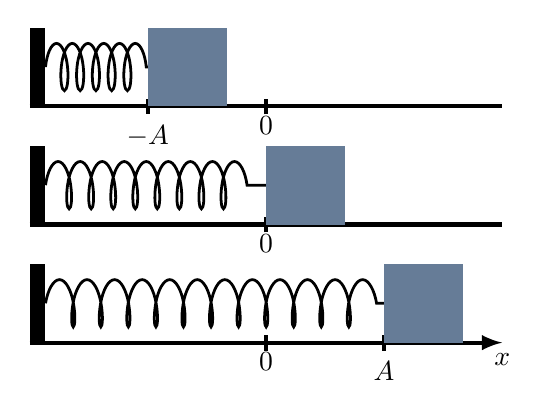
\begin{tikzpicture}[scale=1]
\tikzmath{
\L=2.;
\dx=0.75*\L;
\off=0.5;
\h=1;
}
\scalebox{1}{


\draw[line width=1.5pt] (-1.5*\L,0) -- (1.5*\L,0) ;
\draw[line width=1.5pt] (0,-0.1) -- (0,0.1);
\node[below] at (0,0) {$0$};

\fill (-1.5*\L,0) rectangle (-1.4*\L,\h);
\draw[decoration={aspect=0.3, segment length=2.8mm, amplitude=3mm,coil},decorate,line width=1pt] (-1.4*\L,\h/2) -- (0,\h/2);
%\draw [latex-latex] (-1.4*\L,\h) -- (0,\h) node[midway,above]{$L_0$};
\fill[myblue!60] (0,0) rectangle (\h,\h);

%%%%%%%%%%  top compressed
\begin{scope}[shift={(0,1.5*\h)}]
\draw[line width=1.5pt] (-1.5*\L,0) -- (1.5*\L,0);
\draw[line width=1.5pt] (0,-0.1) -- (0,0.1);
\node[below] at (0,0) {$0$};
\draw[line width=1.5pt] (-\dx,0.1) -- +(0,-0.2)node[below]{$-A$};

\fill (-1.5*\L,0) rectangle (-1.4*\L,\h);
\draw[decoration={aspect=0.3, segment length=2mm, amplitude=3mm,coil},decorate,line width=1pt] (-1.4*\L,\h/2) -- (-\dx,\h/2);
%\draw [color=blue,latex-latex] (-\dx,1.2*\h) -- (0,1.2*\h) node[midway,above]{$x<0$};
\fill[myblue!60] (-\dx,0) rectangle (-\dx+\h,\h);
%\draw[line width=2, -latex, color=myred] (-\dx,\h/2) -- +(1.3,0) node[right] {$\vec F$};

\end{scope}
%%%%%%%%%% bottom extended
\begin{scope}[shift={(0,-1.5*\h)}]
\draw[-latex,line width=1.5pt] (-1.5*\L,0) -- (1.5*\L,0) node[below]{$x$};
\draw[line width=1.5pt] (0,-0.1) -- (0,0.1);
\node[below] at (0,0) {$0$};
\draw[line width=1.5pt] (\dx,0.1) -- +(0,-0.2)node[below]{$A$};

\fill (-1.5*\L,0) rectangle (-1.4*\L,\h);
\draw[decoration={aspect=0.3, segment length=3.5mm, amplitude=3mm,coil},decorate,line width=1pt] (-1.4*\L,\h/2) -- (\dx,\h/2);
%\draw [color=blue,latex-latex] (0,\h) -- (\dx,\h) node[midway,above]{$x>0$};
\fill[myblue!60] (\dx,0) rectangle (\dx+\h,\h);
%\draw[line width=2, -latex, color=myred] (\dx,\h/2) -- +(-1.3,0) node[midway,below=-2pt] {$\vec F$};
\end{scope}

}
\end{tikzpicture}
\captionof*{figure}{\textit{A spring-mass system is a common example of simple harmonic motion.}}
\end{center}


}


%%%%%%%%%%%%%%%%%%%%%%%%%%%%%%%%
\subsection{Integration Constants}
\label{subsec:integrationconstants}
\begin{frame}{Specifying the integration constants}
\begin{align*}
\frac{d^2x}{dt^2}=-\omega^2 x
\end{align*}
\begin{itemize}
\item This is a second order differential equation, so we must specify 2 integration constants.
\item At some time, $t=t_0$, we specify the initial position, $x_0$, and initial velocity, $v_0$.
\item This is enough information to determine $A$ and $\phi$  (say $t_0=0$):
\begin{align*}
x_0&=x(0)=A\cos(\omega t_0 +\phi)=A\cos(\phi)\\
v_0&=v(0)=-A\omega\sin(\omega t_0 +\phi)=-A\omega\sin(\phi)
\end{align*}
\item Similar to:
\begin{align*}
\frac{d^2x}{dt^2}=a \quad\quad x(t)=x_0+v_0t+\frac{1}{2}at^2
\end{align*}
where we specify initial position, $x_0$, and initial velocity, $v_0$
\end{itemize}

\end{frame}


%%%%%%%%%%%%%%%%%%%%%%%%%%%%%%%%


%%%%%%%%%%%%%%%%%%%%%%%%%%%%%%%%



%%%%%%%%%%%%%%%%%%%%%%%%%%%%%%%%
\subsection{SHM in in relation to rotational motion}
\label{subsec:shmplusrm}
\twocolframesf{Back to rotational motion}
{
\begin{itemize}
\item The position of the simple harmonic oscillator is described by the \textbf{same function} as the $x$ or $y$ position of a particle moving around a circle of radius $A$ at constant angular velocity.
\item The phase, $\phi$, tells you where on the circle it started at time $t=0$ (it's like $\theta_0$).
\item Depending on the context, we call, $\omega$, the \textbf{angular frequency} or the \textbf{angular velocity} – we use the terms interchangeably.
\end{itemize}
\begin{align*}
x(t)&=A\cos(\omega t+\phi)=A\cos\left(\theta(t)\right)\\
\theta(t)&=\phi+\omega t
\end{align*}
}
{
\vspace{-1cm}
\begin{center}

\begin{animateinline}[autoplay,loop]{5} % 5 fps, same as 0.2 s transduration

\multiframe{24}{i=1+1}{

\begin{tikzpicture}[scale=1]
\tikzmath{
\R=1.5;
\h=2*\R;
\th=\i*15;
\x=\R*cos(\th);
}

\useasboundingbox (-2*\R,-2.5*\R) rectangle (2*\R,1.5*\R);
\scalebox{1}{
\draw[-latex] (0,0) -- (1.25*\R,0) node[below]{$x$};
\draw[-latex] (0,0) -- (0,1.25*\R) node[left]{$y$};
\draw[line width=1] (0,0) circle (\R);

\fill (\th:\R) circle(2pt);


\draw[-latex,line width=1] (-1.5*\R,-\h) -- (1.5*\R,-\h) node[below]{$x$};

\draw[line width=1] (-\R,-\h+0.1) -- +(0,-0.2) node[below]{$-A$};
\draw[line width=1] (0,-\h+0.1) -- +(0,-0.2) node[below]{$0$};
\draw[line width=1] (\R,-\h+0.1) -- +(0,-0.2) node[below]{$A$};

\fill (\x,-\h) circle(2pt);

\draw[dashed] (\x,-\h) -- (\th:\R);
\draw[-latex, line width=2] (0,0) -- (\th:\R);
\draw[color=red,-latex] (0.7,0) arc(0:\th:0.7);

}
\end{tikzpicture}
}
\end{animateinline}


\captionof*{figure}{\textit{The linear displacement of a spring in SHM is the same as $x$ position of an object in uniform circular motion.}}
\end{center}
}

%%%%%%%%%%%%%%%%%%%%%%%%%%%%%%%%
\begin{frame}{Simple Harmonic Motion}
\begin{itemize}
\item Any physics model that gives:
\begin{align*}
\frac{d^2x}{dt^2}=-\omega^2 x
\end{align*}
is said to correspond to simple harmonic motion and is described by the same math. 
\item SHM arises from physics where there is a \textbf{restoring force} that is \textbf{linearly proportional to displacement}. For example, $F=-kx$.
\item All of the physics is contained in $\omega$, the angular frequency of the motion. 
\item For a mass on a spring:
\begin{align*}
\omega=\sqrt{\frac{k}{m}}
\end{align*}
$\rightarrow$ The frequency of the oscillations depends on how stiff the spring is and how heavy the mass is – nothing else!

\end{itemize}

\end{frame}


%%%%%%%%%%%%%%%%%%%%%%%%%%%%%%%%







%%%%%%%%%%%%%%%%%%%%%%%%%%%%%%%%
\section{Spring Systems}
\label{sec:springs}
\title{Spring Systems}
\institute{Simple Harmonic Motion}
\author{\insertsubsection}


%%%%%%%%%%%%%%%%%%%%%%%%%
\begin{frame}
\titlepage
\thispagestyle{empty}
\end{frame}

%%%%%%%%%%%%%%%%%%%%%%%%





\subsection{Vertical spring system}
\label{subsec:verticalspringsystem}
\twocolframesf{Vertical mass on a spring}
{
\vspace{-0.25cm}
\only<1>{
}

\only<2>{
\begin{itemize}
\item Observations:
\begin{itemize}
\item The mass oscillates about the equilibrium position, not the rest position of the spring.
\item It feels like SHM, so maybe it is?
\end{itemize}
\item The math doesn't quite look like SHM:
\begin{align*}
mg-ky&=ma_y\\
\frac{d^2y}{dt^2}&=g-\frac{k}{m}y
\end{align*}
not the same as:
\begin{align*}
\frac{d^2y}{dt^2}=-\frac{k}{m}y
\end{align*}
\end{itemize}
}

\only<3>{
\begin{itemize}
\item Consider changing coordinate system, so that the origin is located at the point about which the mass oscillates:
\begin{align*}
y'=y-y_0
\end{align*}
\item The extension of the spring is thus:
\begin{align*}
y=y'+y_0
\end{align*}
\item In terms of $y'$, Newton's Second Law reads:
\begin{align*}
\frac{d^2y}{dt^2}&=g-\frac{k}{m}y\\
\frac{d^2(y'+y_0)}{dt^2}&=g-\frac{k}{m}(y'+y_0)
\end{align*}
\end{itemize}
}

\only<4>{
\begin{itemize}
\item Starting from:
\begin{align*}
\frac{d^2(y'+y_0)}{dt^2}&=g-\frac{k}{m}(y'+y_0)\\
\frac{d^2y'}{dt^2}&=g-\frac{k}{m}y'-\frac{k}{m}y_0
\end{align*}
\item At the equilibrium point, the spring is extended by $y_0$, and the spring force is equal to gravity:
\begin{align*}
mg-ky_0 = 0 \quad \rightarrow \quad \frac{k}{m}y_0=g
\end{align*}
and we recover SHM using the $y'$ axis:
\begin{align*}
\frac{d^2y'}{dt^2}&=\frac{k}{m}y'
\end{align*}
\end{itemize}
}

}
{
\vspace{-0.25cm}
\begin{center}
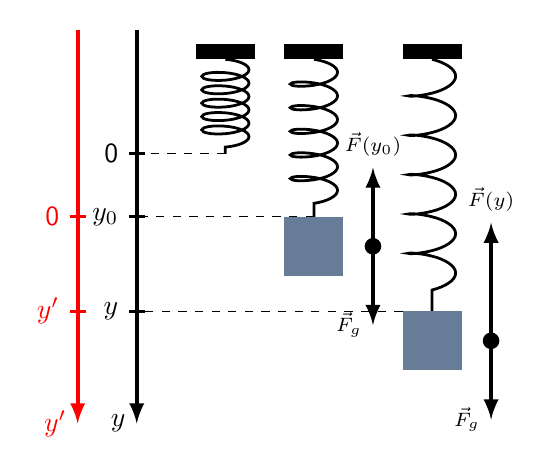
\begin{tikzpicture}[scale=1]
\tikzmath{
\L=2.;
\dx=0.6*\L;
\abox=0.75;
}
\scalebox{1}{

\only<3->{
\draw[-latex,line width=1.5,color=red] (-4*\abox,0.5*\abox) -- +(0,-2.5*\L) node[left]{$y'$};
\draw[line width=1,color=red] (-4*\abox-0.1,-\L) node[left]{0} -- +(0.2,0) ;
\draw[line width=1,color=red] (-4*\abox-0.1,-\L-\dx) node[left]{$y'$} -- +(0.2,0) ;
}

\draw[-latex,line width=1.5] (-3*\abox,0.5*\abox) -- +(0,-2.5*\L) node[left]{$y$};
\draw[dashed] (-1.5*\abox,-\dx) -- (-3*\abox,-\dx);
\draw[line width=1] (-3*\abox-0.1,-\dx) node[left]{0} -- +(0.2,0) ;

\draw[dashed] (0,-\L) -- (-3*\abox,-\L);
\draw[line width=1] (-3*\abox-0.1,-\L) node[left]{$y_0$} -- +(0.2,0) ;

\draw[dashed] (1.5*\abox,-\L-\dx) -- (-3*\abox,-\L-\dx);
\draw[line width=1] (-3*\abox-0.1,-\dx-\L) node[left]{$y$} -- +(0.2,0) ;

%middle
\fill (-0.5*\abox,0) rectangle (0.5*\abox,0.2);
\draw[decoration={aspect=0.3, segment length=3mm, amplitude=3mm,coil},decorate,line width=1pt] (0,0) -- +(0,-\L);
\fill[myblue!60] (-\abox/2,-\L) rectangle +(\abox,-\abox);
%FBD
\coordinate (P) at (\abox,-\L-\abox/2);
\fill (P) circle(3pt);
\draw[-latex,line width=1.5] (P) -- +(0,1) node[above]{\scriptsize $\vec F(y_0)$};
\draw[-latex,line width=1.5] (P) -- +(0,-1) node[left]{\scriptsize $\vec F_g$};


%%%%%%%%%%%  top compressed
\begin{scope}[shift={(-1.5*\abox,0)}]
\fill (-0.5*\abox,0) rectangle (0.5*\abox,0.2);
\draw[decoration={aspect=0.3, segment length=1.7mm, amplitude=3mm,coil},decorate,line width=1pt] (0,0) -- +(0,-\dx);
%\fill[myblue!60] (-\abox/2,-\dx) rectangle +(\abox,-\abox);

\end{scope}

%%%%%%%%%%% bottom extended
\begin{scope}[shift={(2.*\abox,0)}]
\fill (-0.5*\abox,0) rectangle (0.5*\abox,0.2);
\draw[decoration={aspect=0.3, segment length=5mm, amplitude=3mm,coil},decorate,line width=1pt] (0,0) -- +(0,-\dx-\L);
\fill[myblue!60] (-\abox/2,-\dx-\L) rectangle +(\abox,-\abox);
%FBD:
\coordinate (P2) at (\abox,-\L-\dx-\abox/2);
\fill (P2) circle(3pt);
\draw[-latex,line width=1.5] (P2) -- +(0,1.5) node[above]{\scriptsize $\vec F(y)$};
\draw[-latex,line width=1.5] (P2) -- +(0,-1) node[left]{\scriptsize $\vec F_g$};
\end{scope}

}
\end{tikzpicture}
\captionof*{figure}{\textit{A vertical spring-mass system. In the middle position, the force of gravity has the same magnitude as the spring force and the system is in equilibrium.}}
\end{center}

}









%%%%%%%%%%%%%%%%%%%%%%%%%%%%%%%%
\subsection{Constant force + spring force}
\label{subsec:cnsthforceplusspringforce}
\twocolframesf{Constant force + spring force = SHM}
{
\begin{itemize}
\item For a vertical spring-mass, we had an equation of the form:
\begin{align*}
F-kx=m\frac{d^2x}{dt^2}
\end{align*}
where $F$ is a constant force (like gravity).
\item We saw that if we define a new equilibrium position (not the rest position of the spring), then we can recover simple harmonic motion about that point. 
\item With two springs attached to a mass, it's the same idea, and one also recovers SHM $\rightarrow$ in this case the ``effective'' spring constant is $k=k_1+k_2$.
\end{itemize}
}
{
\begin{center}
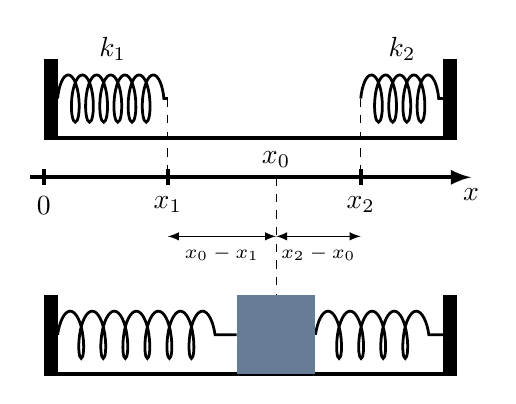
\begin{tikzpicture}[scale=1]
\tikzmath{
\L=1.75;
\dx=0.75*\L;
\off=0.5;
\h=1;
\x1=-0.6*\L;
\x2=0.8*\L;
}
\scalebox{1}{


\draw[line width=1.5pt] (-1.5*\L,0) -- (1.5*\L,0) ;

\draw[line width=1.5pt,-latex] (-1.6*\L,-0.5) -- (1.6*\L,-0.5) node[below]{$x$};
\draw[line width=1.5pt] (-1.5*\L,-0.4) -- +(0,-0.2) node[below] {$0$};

\draw[dashed] (\x1,\h/2) -- (\x1,-0.5);
\draw[line width=1.5pt] (\x1,-0.4) -- +(0,-0.2) node[below] {$x_1$};

\draw[dashed] (\x2,\h/2) -- (\x2,-0.5);
\draw[line width=1.5pt] (\x2,-0.4) -- +(0,-0.2) node[below] {$x_2$};

\fill (-1.5*\L,0) rectangle (-1.4*\L,\h);
\fill (1.4*\L,0) rectangle (1.5*\L,\h);

\draw[decoration={aspect=0.3, segment length=1.8mm, amplitude=3mm,coil},decorate,line width=1pt] (-1.4*\L,\h/2) -- (\x1,\h/2) node[midway, above=10pt]{$k_1$};
\draw[decoration={aspect=0.3, segment length=1.8mm, amplitude=3mm,coil},decorate,line width=1pt] (\x2,\h/2) -- (1.4*\L,\h/2) node[midway, above=10pt]{$k_2$};

\draw[dashed] (-0.1*\L+\h/2,-0.5)node[above]{$x_0$} -- +(0,-2*\h+0.5) ;
\draw[latex-latex] (\x1,-1.25*\h) -- (-0.1*\L+\h/2,-1.25*\h) node[midway,below]{\scriptsize $x_0-x_1$};
\draw[latex-latex] (\x2,-1.25*\h) -- (-0.1*\L+\h/2,-1.25*\h) node[midway,below]{\scriptsize $x_2-x_0$};

\begin{scope}[shift={(0,-3.*\h)}]

\draw[line width=1.5pt] (-1.5*\L,0) -- (1.5*\L,0) ;
\fill (-1.5*\L,0) rectangle (-1.4*\L,\h);
\fill (1.4*\L,0) rectangle (1.5*\L,\h);

\draw[decoration={aspect=0.3, segment length=2.8mm, amplitude=3mm,coil},decorate,line width=1pt] (-1.4*\L,\h/2) -- (-0.1*\L,\h/2);
\draw[decoration={aspect=0.3, segment length=2.8mm, amplitude=3mm,coil},decorate,line width=1pt] (-0.1*\L+\h,\h/2) -- (1.4*\L,\h/2) ;

\fill[myblue!60] (-0.1*\L,0) rectangle +(\h,\h);

\end{scope}

}
\end{tikzpicture}
\captionof*{figure}{\textit{A mass connected to two springs}}
\end{center}
At equilibrium:
\begin{align*}
k_1(x_0-x_1)+k_2(x_2-x_0)=0
\end{align*}

}


%%%%%%%%%%%%%%%%%%%%%%%%%%%%%%%%
%%%%%%%%%%%%%%%%%%%%%%%%%%%%%%%%

\section{Pendulums and Approxomations}
\label{sec:pendulums}
\title{Pendulums and Approxomations}
\institute{Simple Harmonic Motion}
\author{\insertsubsection}


%%%%%%%%%%%%%%%%%%%%%%%%%
\begin{frame}
\titlepage
\thispagestyle{empty}
\end{frame}

%%%%%%%%%%%%%%%%%%%%%%%%
\subsection{Motion of pendulums}
\label{subsec:motionofpendulums}
\twocolframesf{Motion of a pendulum is also SHM}
{
\begin{itemize}
\item The torque from gravity (about the origin) is a \textit{restoring torque} (it tries to bring the pendulum back to equilibrium):
\begin{align*}
\vec \tau_g=-mg\sin\theta L\hat z
\end{align*}
\item Rotational version of Newton's Second Law:
\begin{align*}
\sum \vec \tau=\vec \tau_g&=-mL^2\vec\alpha\\
-mg\sin\theta L &=mL^2\frac{d^2\theta}{dt^2}\\
\frac{d^2\theta}{dt^2}&=-\frac{g}{L}\sin\theta
\end{align*}
not quite SHM...
\end{itemize}
}
{
\vspace{-1cm}
\begin{center}
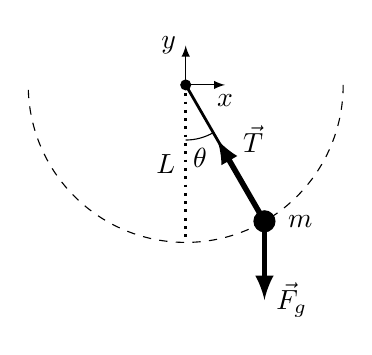
\begin{tikzpicture}[scale=1]
\tikzmath{
\L=2;
\th=30;
}
\scalebox{1}{
\coordinate (P) at (270+\th:\L);
\draw[-latex] (0.0*\L,0) -- +(0.5,0) node[below]{$x$};
\draw[-latex] (0.*\L,0) -- +(0,0.5) node[left]{$y$};
\fill (0,0) circle (2pt);
\fill (P) circle (4pt) node[right=5pt]{$m$};
\draw[line width=1] (0,0) -- (P) ;
\draw[dotted,line width=1] (0,0) -- +(0,-\L) node[midway, left]{$L$};
\draw[dashed] (\L,0) arc (0:-180:\L);

\draw[-latex, line width=2] (P) -- +(90+\th:1.2) node[right=5pt]{$\vec T$};
\draw[-latex, line width=2] (P) -- +(0,-1) node[right]{$\vec F_g$};

\draw (0,-0.7) arc (270:270+\th:0.7) node[midway,below]{$\theta$};

}
\end{tikzpicture}
\captionof*{figure}{\textit{Modeling a pendulum, using torque from gravity.}}
\end{center}
\only<2>{
\vspace{-0.5cm}
\begin{block}{Small angle approximation}
To get SHM, need to approximate $\sin\theta\sim\theta$, then:
\begin{align*}
\frac{d^2\theta}{dt^2}&\sim -\frac{g}{L}\theta \quad\rightarrow\quad \omega=\sqrt{\frac{g}{L}}\\
\therefore \theta(t) &= A\cos(\omega t+\phi)
\end{align*}
\end{block}
}
}


%%%%%%%%%%%%%%%%%%%%%%%%%%%%%%%%
\subsection{Small angle approxomations}
\label{subsec:smallangles}
\begin{frame}{What does it mean for $\theta$ to be small?}
\begin{itemize}
\item How small is small?
\item You try it out on your calculator...  has to be in radians for this to work...
\item If the angle is too big, then it's not SHM anymore. We'll do a lab next semester to figure this out. It turns out that SHM is a very good approximation even to relatively large angles.
\end{itemize}
\begin{columns}

\column{0.5\textwidth}
\begin{center}
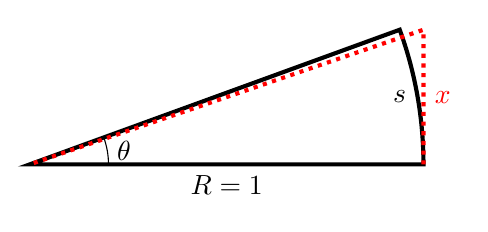
\begin{tikzpicture}[scale=1]
\tikzmath{
\L=5;
\th=20;
\h=\L*sin(\th);
}
\scalebox{1}{
\draw[line width=1.5] (0,0) -- (\L,0) node[midway,below] {$R=1$} arc(0:\th:\L) node[midway,left]{$s$}-- cycle;
\draw[line width=1.5,color=red,dotted] (\L,0) -- +(0,\h) node[midway,right]{$x$} -- (0,0);

\draw (1,0) arc(0:\th:1) node[midway,right]{$\theta$};
}
\end{tikzpicture}
\captionof*{figure}{\textit{The small angle approximation.}}
\end{center}
\column{0.5\textwidth}
\begin{align*}
\textcolor{red}{x=\sin\theta}\\
s=R\theta=\theta
\end{align*}
The approximation is that $s\sim x$.
\end{columns}
\end{frame}


%%%%%%%%%%%%%%%%%%%%%%%%%%%%%%%%
\subsection{Physical pendulums}
\label{subsec:physicalpendulums}
\twocolframesf{Physical pendulum}
{
\begin{itemize}
\item Same idea as ``simple'' pendulum.
\item Object with moment of inertia, $I$, instead of a point mass:
\begin{align*}
\vec \tau_g&=I\vec\alpha\\
-mg\sin\theta h &=I\frac{d^2\theta}{dt^2}\\
\omega&=\sqrt{\frac{mgh}{I}}
\end{align*}
\end{itemize}
}
{
\vspace{-1cm}
\begin{center}
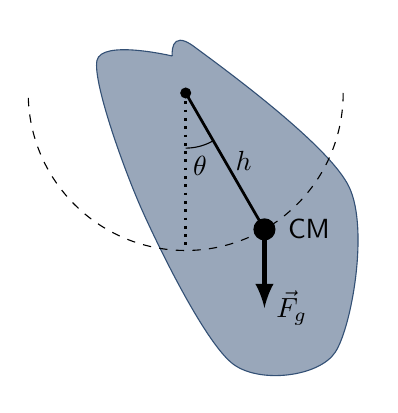
\begin{tikzpicture}[scale=1]
\tikzmath{
\L=2;
\th=30;
}
\scalebox{1}{
\coordinate (P) at (270+\th:\L);

\fill[color=myblue!40,draw=myblue!80] plot[smooth] coordinates {(110:0.25*\L) (80:0.3*\L) (-30:1.2*\L) (-60:1.9*\L) (-80:1.75*\L) (250:0.8*\L) (160:0.6*\L) (110:0.25*\L)};


\node[right=5pt] at (P) {CM};
\fill (0,0) circle (2pt);
\fill (P) circle (4pt);
\draw[line width=1] (0,0) -- (P) node[midway,right]{$h$};
\draw[dotted,line width=1] (0,0) -- +(0,-\L);
\draw[dashed] (\L,0) arc (0:-180:\L);


\draw[-latex, line width=2] (P) -- +(0,-1) node[right]{$\vec F_g$};

\draw (0,-0.7) arc (270:270+\th:0.7) node[midway,below]{$\theta$};


}
\end{tikzpicture}
\captionof*{figure}{\textit{A physical pendulum swings because of the torque from gravity, exerted at the CM.}}
\end{center}

}


%%%%%%%%%%%%%%%%%%%%%%%%%%%%%%%%
\subsection{Group activity}
\label{subsec:}
\begin{frame}{Group activity: Pendulum}
What length to make the string to have a period of \SI{1}{s}?
\begin{align*}
\omega &=\sqrt{\frac{g}{L}}\\
T &=\frac{2\pi}{\omega}
\end{align*}

\end{frame}


%%%%%%%%%%%%%%%%%%%%%%%%%%%%%%%%


%%%%%%%%%%%%%%%%%%%%%%%%%%%%%%%%
\subsection{SHM is everywhere!}
\label{subsec:shmiseverywhere}
\begin{frame}{Simple Harmonic Motion is everywhere!}
\begin{itemize}
\item You get SHM any time you have a ``linear restoring force'' (or torque).
\item Everything is linear on small scale, so this can apply to many things.
\item Next semester, we'll look at waves propagating in a medium, and we'll see that we can model the small deformations in the medium as SHM.
\end{itemize}


\begin{columns}

\column{0.3\textwidth}
\capfig{1}{../figures/SimpleHarmonicMotion/ripples}{Surface waves on a pond can be modeled using SHM.}
\column{0.7\textwidth}
\begin{center}

\begin{animateinline}[autoplay,loop]{10} % 5 fps, same as 0.2 s transduration

\multiframe{24}{i=1+1}{

\begin{tikzpicture}[scale=1]
\tikzmath{
\h=2;
\L=8;
\wl=\L/2;%wavelength
\om=2*pi/\wl;%effective frequency
\phas=2*pi/24*\i;
\Ax=0.75;
}

\useasboundingbox (0,-2*\Ax) rectangle (\L,\h+0.2);
\scalebox{1}{

\fill (0,\h) rectangle +(\L,0.2);
\draw[trig format=rad, line width=2] plot[ domain=0:\L, variable=\x, samples=100] ({\x},{\Ax*cos(\om*\x-\phas)});
 
  \foreach \xl in {0.2,0.4,0.6,0.8}{
  \tikzmath{
    \xp=\xl*\L;
    \yp=\Ax*cos((\om*\xp-\phas)*180/pi);%needs to be in degrees...
    \lcy=(\h-\yp);
  }
  \coordinate (P) at (\xp,\yp);
  \draw[decoration={aspect=0.3, segment length=\lcy mm, amplitude=3mm,coil},decorate,line width=1pt] (\xp,\h) -- (P);
  \fill (P) circle (4pt);
}
  
  
}
\end{tikzpicture}
}
\end{animateinline}

\captionof*{figure}{\textit{A wave going through a medium modeled with particles in the medium acting as simple harmonic oscillators.}}
\end{center}

\end{columns}
\end{frame}

%%%%%%%%%%%%%%%%%%%%%%%%%%%%%%%%



%%%%%%%%%%%%%%%%%%%%%%%%%%%%%%%%



%%%%%%%%%%%%%%%%%%%%%%%%%%%%%%%%



%%%%%%%%%%%%%%%%%%%%%%%%%%%%%%%%



%%%%%%%%%%%%%%%%%%%%%%%%%%%%%%%%



%%%%%%%%%%%%%%%%%%%%%%%%%%%%%%%%



%%%%%%%%%%%%%%%%%%%%%%%%%%%%%%%%



%%%%%%%%%%%%%%%%%%%%%%%%%%%%%%%%



%%%%%%%%%%%%%%%%%%%%%%%%%%%%%%%%



%%%%%%%%%%%%%%%%%%%%%%%%%%%%%%%%



%%%%%%%%%%%%%%%%%%%%%%%%%%%%%%%%



%%%%%%%%%%%%%%%%%%%%%%%%%%%%%%%%



%%%%%%%%%%%%%%%%%%%%%%%%%%%%%%%%



%%%%%%%%%%%%%%%%%%%%%%%%%%%%%%%%



%%%%%%%%%%%%%%%%%%%%%%%%%%%%%%%%



%%%%%%%%%%%%%%%%%%%%%%%%%%%%%%%%



%%%%%%%%%%%%%%%%%%%%%%%%%%%%%%%%



%%%%%%%%%%%%%%%%%%%%%%%%%%%%%%%%



%%%%%%%%%%%%%%%%%%%%%%%%%%%%%%%%



%%%%%%%%%%%%%%%%%%%%%%%%%%%%%%%%



%%%%%%%%%%%%%%%%%%%%%%%%%%%%%%%%






\end{document}